\PassOptionsToPackage{unicode=true}{hyperref} % options for packages loaded elsewhere
\PassOptionsToPackage{hyphens}{url}
%
\documentclass[english,man,floatsintext]{apa6}
\usepackage{lmodern}
\usepackage{amssymb,amsmath}
\usepackage{ifxetex,ifluatex}
\usepackage{fixltx2e} % provides \textsubscript
\ifnum 0\ifxetex 1\fi\ifluatex 1\fi=0 % if pdftex
  \usepackage[T1]{fontenc}
  \usepackage[utf8]{inputenc}
  \usepackage{textcomp} % provides euro and other symbols
\else % if luatex or xelatex
  \usepackage{unicode-math}
  \defaultfontfeatures{Ligatures=TeX,Scale=MatchLowercase}
\fi
% use upquote if available, for straight quotes in verbatim environments
\IfFileExists{upquote.sty}{\usepackage{upquote}}{}
% use microtype if available
\IfFileExists{microtype.sty}{%
\usepackage[]{microtype}
\UseMicrotypeSet[protrusion]{basicmath} % disable protrusion for tt fonts
}{}
\IfFileExists{parskip.sty}{%
\usepackage{parskip}
}{% else
\setlength{\parindent}{0pt}
\setlength{\parskip}{6pt plus 2pt minus 1pt}
}
\usepackage{hyperref}
\hypersetup{
            pdftitle={Behavioral, neural, and psychiatric correlates of social feedback},
            pdfauthor={Brent I. Rappaport1, Autumn Kujawa2, Kodi B. Arfer3, Samantha Pegg2, Danielle Kelly4, Joan L. Luby4, \& Deanna M. Barch1,4,5},
            pdfkeywords={social feedback, ERP, depression, social anxiety, reward, reward positivity, feedback negativity},
            pdfborder={0 0 0},
            breaklinks=true}
\urlstyle{same}  % don't use monospace font for urls
\usepackage{graphicx,grffile}
\makeatletter
\def\maxwidth{\ifdim\Gin@nat@width>\linewidth\linewidth\else\Gin@nat@width\fi}
\def\maxheight{\ifdim\Gin@nat@height>\textheight\textheight\else\Gin@nat@height\fi}
\makeatother
% Scale images if necessary, so that they will not overflow the page
% margins by default, and it is still possible to overwrite the defaults
% using explicit options in \includegraphics[width, height, ...]{}
\setkeys{Gin}{width=\maxwidth,height=\maxheight,keepaspectratio}
\setlength{\emergencystretch}{3em}  % prevent overfull lines
\providecommand{\tightlist}{%
  \setlength{\itemsep}{0pt}\setlength{\parskip}{0pt}}
\setcounter{secnumdepth}{0}

% set default figure placement to htbp
\makeatletter
\def\fps@figure{htbp}
\makeatother

% Manuscript styling
\usepackage{upgreek}
\captionsetup{font=singlespacing,justification=justified}

% Table formatting
\usepackage{longtable}
\usepackage{lscape}
% \usepackage[counterclockwise]{rotating}   % Landscape page setup for large tables
\usepackage{multirow}		% Table styling
\usepackage{tabularx}		% Control Column width
\usepackage[flushleft]{threeparttable}	% Allows for three part tables with a specified notes section
\usepackage{threeparttablex}            % Lets threeparttable work with longtable

% Create new environments so endfloat can handle them
% \newenvironment{ltable}
%   {\begin{landscape}\begin{center}\begin{threeparttable}}
%   {\end{threeparttable}\end{center}\end{landscape}}
\newenvironment{lltable}{\begin{landscape}\begin{center}\begin{ThreePartTable}}{\end{ThreePartTable}\end{center}\end{landscape}}

% Enables adjusting longtable caption width to table width
% Solution found at http://golatex.de/longtable-mit-caption-so-breit-wie-die-tabelle-t15767.html
\makeatletter
\newcommand\LastLTentrywidth{1em}
\newlength\longtablewidth
\setlength{\longtablewidth}{1in}
\newcommand{\getlongtablewidth}{\begingroup \ifcsname LT@\roman{LT@tables}\endcsname \global\longtablewidth=0pt \renewcommand{\LT@entry}[2]{\global\advance\longtablewidth by ##2\relax\gdef\LastLTentrywidth{##2}}\@nameuse{LT@\roman{LT@tables}} \fi \endgroup}

% \setlength{\parindent}{0.5in}
% \setlength{\parskip}{0pt plus 0pt minus 0pt}

% Overwrite redefinition of paragraph and subparagraph by the default LaTeX template
% See https://github.com/crsh/papaja/issues/292
\makeatletter
\renewcommand{\paragraph}{\@startsection{paragraph}{4}{\parindent}%
  {0\baselineskip \@plus 0.2ex \@minus 0.2ex}%
  {-1em}%
  {\normalfont\normalsize\bfseries\itshape\typesectitle}}

\renewcommand{\subparagraph}[1]{\@startsection{subparagraph}{5}{1em}%
  {0\baselineskip \@plus 0.2ex \@minus 0.2ex}%
  {-\z@\relax}%
  {\normalfont\normalsize\itshape\hspace{\parindent}{#1}\textit{\addperi}}{\relax}}
\makeatother

% \usepackage{etoolbox}
\makeatletter
\patchcmd{\HyOrg@maketitle}
  {\section{\normalfont\normalsize\abstractname}}
  {\section*{\normalfont\normalsize\abstractname}}
  {}{\typeout{Failed to patch abstract.}}
\patchcmd{\HyOrg@maketitle}
  {\section{\protect\normalfont{\@title}}}
  {\section*{\protect\normalfont{\@title}}}
  {}{\typeout{Failed to patch title.}}
\makeatother
\shorttitle{Correlates of social feedback}
\keywords{social feedback, ERP, depression, social anxiety, reward, reward positivity, feedback negativity\newline\indent Word count: X}
\usepackage{lineno}

\linenumbers
\usepackage{csquotes}
\ifnum 0\ifxetex 1\fi\ifluatex 1\fi=0 % if pdftex
  \usepackage[shorthands=off,main=english]{babel}
\else
  % load polyglossia as late as possible as it *could* call bidi if RTL lang (e.g. Hebrew or Arabic)
  \usepackage{polyglossia}
  \setmainlanguage[]{english}
\fi

\title{Behavioral, neural, and psychiatric correlates of social feedback}
\author{Brent I. Rappaport\textsuperscript{1}, Autumn Kujawa\textsuperscript{2}, Kodi B. Arfer\textsuperscript{3}, Samantha Pegg\textsuperscript{2}, Danielle Kelly\textsuperscript{4}, Joan L. Luby\textsuperscript{4}, \& Deanna M. Barch\textsuperscript{1,4,5}}
\date{}


\authornote{

1 Psychological \& Brain Science, Washington University in St.~Louis, St.~Louis, MO\\
2 Department of Psychology \& Human Development, Vanderbilt University, Nashville, TN\\
3 Center for HIV Identification, Prevention, and Treatment Services, University of California, Los Angeles, Los Angeles, CA\\
4 Department of Psychiatry, School of Medicine, Washington University in St.~Louis, St.~Louis, MO\\
5 Department of Radiology, School of Medicine, Washington University in St.~Louis, St.~Louis, MO\\

The authors made the following contributions. Brent I. Rappaport: Conceptualization, Formal Analysis, Writing - Original Draft Preparation, Writing - Review \& Editing; Autumn Kujawa: Methodology, Conceptualization, Writing - Review \& Editing; Kodi B. Arfer: Software, Writing - Review \& Editing; Samantha Pegg: Formal Analysis, Writing - Review \& Editing; Danielle Kelly: Writing - Review \& Editing, Supervision, Resources, Funding acquisition; Joan L. Luby: Resources, Funding acquisition, Writing - Review \& Editing; Deanna M. Barch: Conceptualization, Supervision, Resources, Funding acquisition, Writing - Review \& Editing.

Correspondence concerning this article should be addressed to Brent I. Rappaport, One Brookings Drive St.~Louis, MO 63130. E-mail: \href{mailto:brappaport@wustl.edu}{\nolinkurl{brappaport@wustl.edu}}

}

\affiliation{\vspace{0.5cm}\textsuperscript{1} Psychological \& Brain Science, Washington University in St.~Louis\\\textsuperscript{2} Department of Psychology \& Human Development, Vanderbilt University\\\textsuperscript{3} Center for HIV Identification, Prevention, and Treatment Services, University of California\\\textsuperscript{4} Department of Psychiatry, School of Medicine, Washington University in St.~Louis\\\textsuperscript{5} Department of Radiology, School of Medicine, Washington University in St.~Louis}

\begin{document}
\maketitle

\begin{table}[tbp]

\begin{center}
\begin{threeparttable}

\caption{\label{tab:unnamed-chunk-1}Demographics of study sample}

\begin{tabular}{ll}
\toprule
Variable & \multicolumn{1}{c}{Sample (N=114)}\\
\midrule
Age & 18.52 (1.1)\\
SES (income to need) & 3.61 (2.35)\\
Sex (female) & 57 (50\%)\\
White or Caucasian & 69 (60.53\%)\\
Black or African American & 33 (28.95\%)\\
Multiracial & 12 (10.53\%)\\
Hispanic & 3 (2.63\%)\\
Recent psychotropic medication use & 13 (12.38\%)\\
\bottomrule
\addlinespace
\end{tabular}

\begin{tablenotes}[para]
\normalsize{\textit{Note.} N=9 missing recent psychotropic medication use. Mean (SD) for continuous variables or N (\%) for categorical variables presented.}
\end{tablenotes}

\end{threeparttable}
\end{center}

\end{table}

\begin{lltable}

\begin{TableNotes}[para]
\normalsize{\textit{Note.} Correlations coefficients (r) are presented in the upper diagonal, while residual standard errors (rse) are presented in the lower diagonal}
\end{TableNotes}

\begin{longtable}{llllllll}\noalign{\getlongtablewidth\global\LTcapwidth=\longtablewidth}
\caption{\label{tab:unnamed-chunk-2}Correlations between variables of interest}\\
\toprule
 & \multicolumn{1}{c}{Mean SD} & \multicolumn{1}{c}{RewP} & \multicolumn{1}{c}{FN} & \multicolumn{1}{c}{Reward Bias} & \multicolumn{1}{c}{Loss Avoidance} & \multicolumn{1}{c}{Depression} & \multicolumn{1}{c}{Social Anxiety}\\
\midrule
\endfirsthead
\caption*{\normalfont{Table \ref{tab:unnamed-chunk-2} continued}}\\
\toprule
 & \multicolumn{1}{c}{Mean SD} & \multicolumn{1}{c}{RewP} & \multicolumn{1}{c}{FN} & \multicolumn{1}{c}{Reward Bias} & \multicolumn{1}{c}{Loss Avoidance} & \multicolumn{1}{c}{Depression} & \multicolumn{1}{c}{Social Anxiety}\\
\midrule
\endhead
RewP & 0 (1.02) & — & 0.829 & 0.013 & 0.032 & -0.08 & 0.049\\
FN & 0 (1.01) & 0.03 & — & 0.028 & 0.196 & -0.007 & 0.116\\
Reward Bias & 0.19 (0.57) & 0.1 & 0.099 & — & -0.053 & 0.074 & 0.024\\
Loss Avoidance & 0.25 (0.61) & 0.107 & 0.107 & 0.1 & — & 0.16 & 0.04\\
Depression & 11.43 (12.91) & 0.096 & 0.096 & 0.098 & 0.096 & — & 0.54\\
Social Anxiety & 4.72 (4.18) & 0.095 & 0.094 & 0.104 & 0.101 & 0.067 & —\\
\bottomrule
\addlinespace
\insertTableNotes
\end{longtable}

\end{lltable}

\begin{table}[tbp]

\begin{center}
\begin{threeparttable}

\caption{\label{tab:unnamed-chunk-5}Multiple regressions of RewP/FN predicted by behavioral reward bias and loss avoidance and psychopathology}

\begin{tabular}{lcccccc}
\toprule
 \multicolumn{1}{c}{Predictors} & \multicolumn{3}{c}{RewP} & \multicolumn{3}{c}{FN} \\
\cmidrule(r){1-1} \cmidrule(r){2-4} \cmidrule(r){5-7}
  & $\beta$ & CI & $p$ & $\beta$ & CI & $p$\\
\midrule
Reward bias and loss avoidance &  &  &  &  &  & \\
\ \ \ Intercept & 0.07 & (-0.244, 0.386) & 0.66 & 0.04 & (-0.282, 0.353) & 0.82\\
\ \ \ Reward Bias & -0.02 & (-0.235, 0.189) & 0.83 & 0.02 & (-0.186, 0.223) & 0.86\\
\ \ \ Loss Avoidance & 0.12 & (-0.119, 0.349) & 0.33 & 0.25 & (0.016, 0.487) & 0.04\\
\ \ \ Age & 0.06 & (-0.13, 0.254) & 0.52 & 0.01 & (-0.181, 0.203) & 0.91\\
\ \ \ Sex & -0.10 & (-0.481, 0.277) & 0.59 & 0.00 & (-0.376, 0.383) & 0.98\\
\ \ \ Black or AA & -0.12 & (-0.6, 0.365) & 0.63 & -0.13 & (-0.615, 0.357) & 0.60\\
\ \ \ Multiracial & 0.02 & (-0.661, 0.705) & 0.95 & -0.15 & (-0.831, 0.536) & 0.67\\
\ \ \ Hispanic & 0.44 & (-0.8, 1.67) & 0.49 & 0.56 & (-0.674, 1.793) & 0.37\\
\ \ \ SES & 0.26 & (0.02, 0.495) & 0.03 & 0.17 & (-0.073, 0.405) & 0.17\\
Psychopathology &  &  &  &  &  & \\
\ \ \ Intercept & 0.07 & (-0.244, 0.387) & 0.66 & 0.07 & (-0.249, 0.395) & 0.65\\
\ \ \ Depression & -0.12 & (-0.367, 0.124) & 0.33 & -0.09 & (-0.334, 0.162) & 0.49\\
\ \ \ Social Anxiety & 0.11 & (-0.115, 0.336) & 0.33 & 0.16 & (-0.069, 0.389) & 0.17\\
\ \ \ Age & 0.04 & (-0.155, 0.232) & 0.69 & -0.02 & (-0.218, 0.178) & 0.84\\
\ \ \ Sex & -0.11 & (-0.488, 0.268) & 0.56 & -0.05 & (-0.439, 0.331) & 0.78\\
\ \ \ Black or AA & -0.12 & (-0.596, 0.365) & 0.64 & -0.14 & (-0.63, 0.35) & 0.57\\
\ \ \ Multiracial & 0.04 & (-0.653, 0.731) & 0.91 & -0.20 & (-0.903, 0.508) & 0.58\\
\ \ \ Hispanic & 0.50 & (-0.735, 1.746) & 0.42 & 0.58 & (-0.68, 1.848) & 0.36\\
\ \ \ SES & 0.20 & (-0.011, 0.417) & 0.06 & 0.08 & (-0.143, 0.293) & 0.50\\
\bottomrule
\end{tabular}

\end{threeparttable}
\end{center}

\end{table}

\begin{table}[tbp]

\begin{center}
\begin{threeparttable}

\caption{\label{tab:unnamed-chunk-6}Multiple regressions of Reward bias/loss avoidance predicted by psychopathology}

\begin{tabular}{lcccccc}
\toprule
 \multicolumn{1}{c}{ } & \multicolumn{3}{c}{Reward bias} & \multicolumn{3}{c}{Loss avoidance} \\
\cmidrule(r){1-1} \cmidrule(r){2-4} \cmidrule(r){5-7}
  & $\beta$ & CI & $p$ & $\beta$ & CI & $p$\\
\midrule
Intercept & -0.01 & (-0.358, 0.332) & 0.94 & 0.22 & (-0.117, 0.562) & 0.20\\
Depression & 0.07 & (-0.18, 0.312) & 0.60 & 0.20 & (-0.037, 0.438) & 0.10\\
Social Anxiety & -0.02 & (-0.262, 0.216) & 0.85 & -0.04 & (-0.269, 0.182) & 0.70\\
Age & -0.09 & (-0.29, 0.106) & 0.36 & -0.06 & (-0.255, 0.127) & 0.51\\
Sex & -0.18 & (-0.614, 0.265) & 0.43 & -0.21 & (-0.62, 0.197) & 0.30\\
Black or AA & 0.21 & (-0.296, 0.709) & 0.42 & -0.21 & (-0.728, 0.304) & 0.42\\
Multiracial & 0.51 & (-0.244, 1.268) & 0.18 & -0.49 & (-1.165, 0.179) & 0.15\\
Hispanic & -0.52 & (-1.762, 0.728) & 0.41 & -0.13 & (-1.317, 1.059) & 0.83\\
SES & 0.23 & (0.005, 0.461) & 0.04 & -0.35 & (-0.581, -0.119) & 0.00\\
\bottomrule
\end{tabular}

\end{threeparttable}
\end{center}

\end{table}

\begin{table}[tbp]

\begin{center}
\begin{threeparttable}

\caption{\label{tab:unnamed-chunk-7}Model fit of SEM model of hypotheses}

\begin{tabular}{lcc}
\toprule
Fit measure & Simplified model & Full model\\
\midrule
chisq & 18.97 & 7.11\\
df & 12.00 & 4.00\\
pvalue & 0.09 & 0.13\\
cfi & 0.96 & 0.98\\
rmsea & 0.07 & 0.08\\
srmr & 0.06 & 0.03\\
aic & 2,372.37 & 2,376.52\\
bic & 2,413.42 & 2,439.45\\
\bottomrule
\addlinespace
\end{tabular}

\begin{tablenotes}[para]
\normalsize{\textit{Note.} Delta chi\textasciicircum{}2 = 13.61}
\end{tablenotes}

\end{threeparttable}
\end{center}

\end{table}

\begin{figure}
\includegraphics[width=1\linewidth]{../figures/IG_PILT} \caption{Depiction of Island Getaway ERP task trial and schematic of Probabilistic Incentive Learning Task (PILT)}(\#fig:Figure 1)
\end{figure}

\begin{verbatim}
## Warning: attributes are not identical across measure variables;
## they will be dropped
\end{verbatim}

\begin{figure}

{\centering 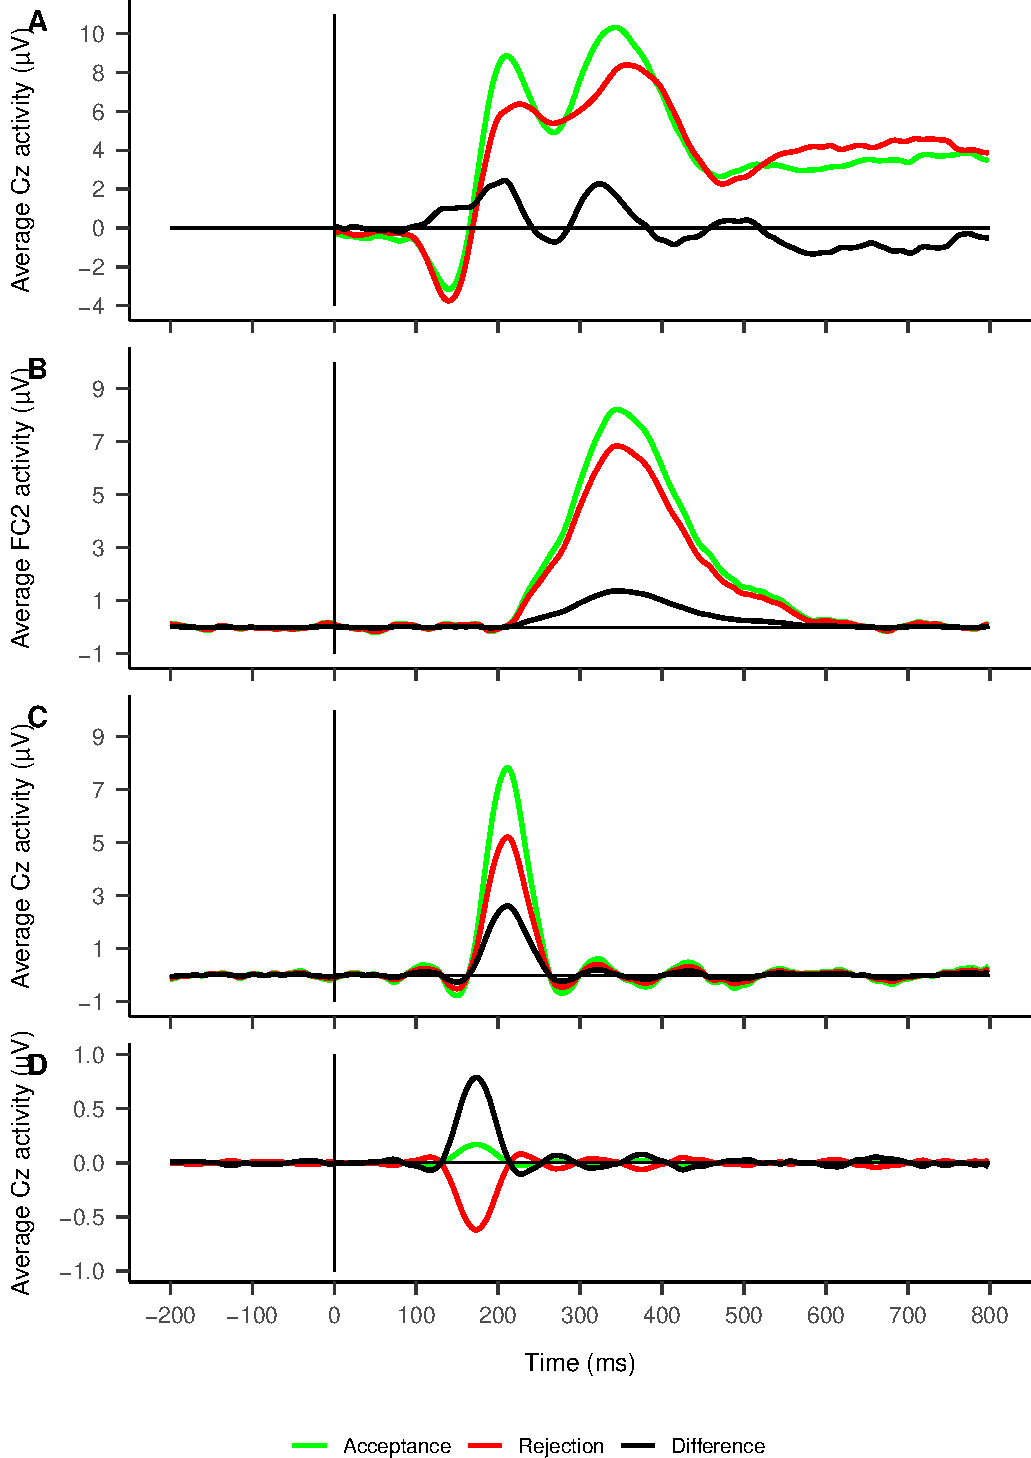
\includegraphics[width=1\linewidth]{DISS_tablesfigures_files/figure-latex/Facet plots together-1} 

}

\caption{ERP waveforms to acceptance and rejection feedback}(\#fig:Facet plots together)
\end{figure}

\hypertarget{figure-3}{%
\subsection{Figure 3}\label{figure-3}}

\begin{figure}

{\centering 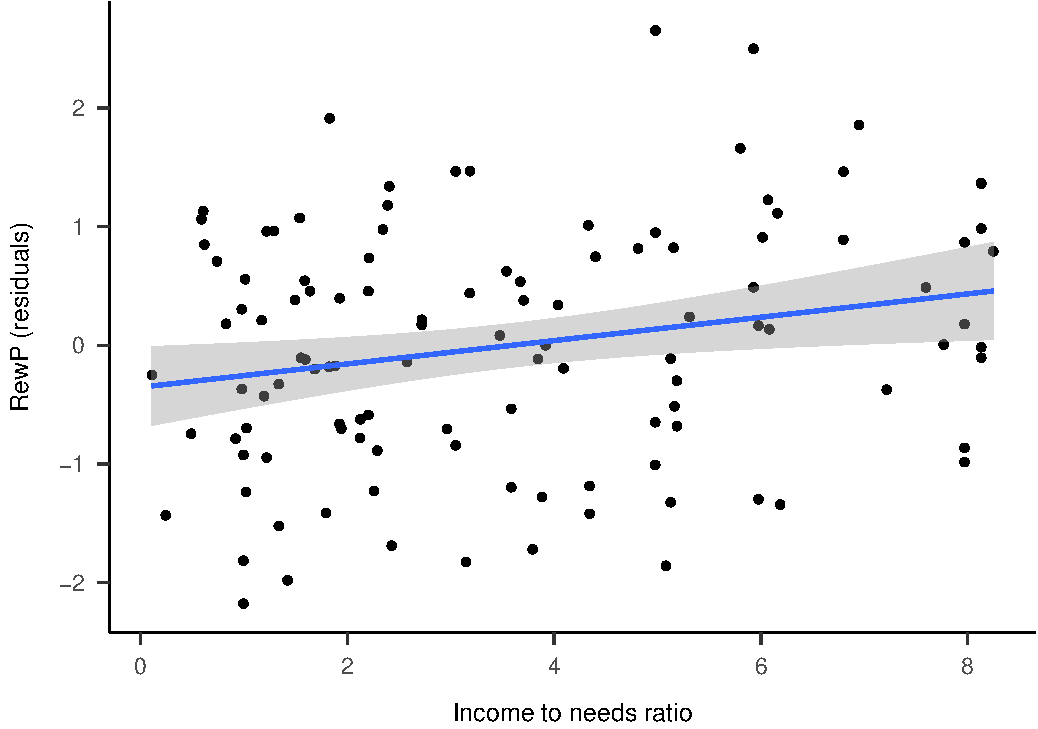
\includegraphics[width=1\linewidth]{DISS_tablesfigures_files/figure-latex/I2N plot-1} 

}

\caption{RewP to social acceptance and income to needs ratio}(\#fig:I2N plot)
\end{figure}

\newpage

\hypertarget{supplement}{%
\section{Supplement}\label{supplement}}

\begin{table}[tbp]

\begin{center}
\begin{threeparttable}

\caption{\label{tab:unnamed-chunk-8}Multiple regressions of RewP/FN predicted by behavioral reward bias and loss avoidance covarying for accuracy}

\begin{tabular}{lcccccc}
\toprule
 \multicolumn{1}{c}{ } & \multicolumn{3}{c}{RewP} & \multicolumn{3}{c}{FN} \\
\cmidrule(r){1-1} \cmidrule(r){2-4} \cmidrule(r){5-7}
  & $\beta$ & CI & $p$ & $\beta$ & CI & $p$\\
\midrule
Intercept & 0.12 & (-0.537, 0.774) & 0.72 & 0.22 & (-0.443, 0.891) & 0.51\\
Reward Bias & 0.02 & (-0.211, 0.257) & 0.85 & 0.06 & (-0.154, 0.284) & 0.56\\
Loss Avoidance & 0.12 & (-0.122, 0.355) & 0.33 & 0.24 & (0.002, 0.486) & 0.05\\
PILT-P Accuracy & -0.29 & (-0.895, 0.311) & 0.33 & -0.37 & (-0.924, 0.192) & 0.19\\
PILT-N Accuracy & 0.26 & (-0.321, 0.832) & 0.37 & 0.23 & (-0.347, 0.799) & 0.42\\
Age & 0.07 & (-0.123, 0.268) & 0.46 & 0.02 & (-0.181, 0.211) & 0.88\\
Sex & -0.13 & (-0.51, 0.256) & 0.51 & -0.02 & (-0.402, 0.367) & 0.93\\
Black or AA & -0.23 & (-0.763, 0.298) & 0.39 & -0.26 & (-0.785, 0.268) & 0.33\\
Multiracial & 0.08 & (-0.613, 0.764) & 0.83 & -0.09 & (-0.775, 0.599) & 0.80\\
Hispanic & 0.38 & (-0.855, 1.615) & 0.54 & 0.51 & (-0.72, 1.741) & 0.41\\
SES & 0.24 & (0.004, 0.485) & 0.05 & 0.16 & (-0.086, 0.396) & 0.20\\
\bottomrule
\end{tabular}

\end{threeparttable}
\end{center}

\end{table}

\begin{table}[tbp]

\begin{center}
\begin{threeparttable}

\caption{\label{tab:unnamed-chunk-9}Multiple regressions of RewP/FN predicted by behavioral reward bias and loss avoidance and psychopathology covarying for recent psychotropic medication use}

\begin{tabular}{lcccccc}
\toprule
 \multicolumn{1}{c}{Predictors} & \multicolumn{3}{c}{RewP} & \multicolumn{3}{c}{FN} \\
\cmidrule(r){1-1} \cmidrule(r){2-4} \cmidrule(r){5-7}
  & $\beta$ & CI & $p$ & $\beta$ & CI & $p$\\
\midrule
Reward bias and loss avoidance &  &  &  &  &  & \\
\ \ \ Intercept & 0.07 & (-0.244, 0.386) & 0.66 & 0.04 & (-0.282, 0.353) & 0.82\\
\ \ \ Reward Bias & -0.02 & (-0.235, 0.189) & 0.83 & 0.02 & (-0.186, 0.223) & 0.86\\
\ \ \ Loss Avoidance & 0.12 & (-0.119, 0.349) & 0.33 & 0.25 & (0.016, 0.487) & 0.04\\
\ \ \ Age & 0.06 & (-0.13, 0.254) & 0.52 & 0.01 & (-0.181, 0.203) & 0.91\\
\ \ \ Sex & -0.10 & (-0.481, 0.277) & 0.59 & 0.00 & (-0.376, 0.383) & 0.98\\
\ \ \ Black or AA & -0.12 & (-0.6, 0.365) & 0.63 & -0.13 & (-0.615, 0.357) & 0.60\\
\ \ \ Multiracial & 0.02 & (-0.661, 0.705) & 0.95 & -0.15 & (-0.831, 0.536) & 0.67\\
\ \ \ Hispanic & 0.44 & (-0.8, 1.67) & 0.49 & 0.56 & (-0.674, 1.793) & 0.37\\
\ \ \ SES & 0.26 & (0.02, 0.495) & 0.03 & 0.17 & (-0.073, 0.405) & 0.17\\
Psychopathology &  &  &  &  &  & \\
\ \ \ Intercept & 0.07 & (-0.244, 0.387) & 0.66 & 0.07 & (-0.249, 0.395) & 0.65\\
\ \ \ Depression & -0.12 & (-0.367, 0.124) & 0.33 & -0.09 & (-0.334, 0.162) & 0.49\\
\ \ \ Social Anxiety & 0.11 & (-0.115, 0.336) & 0.33 & 0.16 & (-0.069, 0.389) & 0.17\\
\ \ \ Age & 0.04 & (-0.155, 0.232) & 0.69 & -0.02 & (-0.218, 0.178) & 0.84\\
\ \ \ Sex & -0.11 & (-0.488, 0.268) & 0.56 & -0.05 & (-0.439, 0.331) & 0.78\\
\ \ \ Black or AA & -0.12 & (-0.596, 0.365) & 0.64 & -0.14 & (-0.63, 0.35) & 0.57\\
\ \ \ Multiracial & 0.04 & (-0.653, 0.731) & 0.91 & -0.20 & (-0.903, 0.508) & 0.58\\
\ \ \ Hispanic & 0.50 & (-0.735, 1.746) & 0.42 & 0.58 & (-0.68, 1.848) & 0.36\\
\ \ \ SES & 0.20 & (-0.011, 0.417) & 0.06 & 0.08 & (-0.143, 0.293) & 0.50\\
\bottomrule
\end{tabular}

\end{threeparttable}
\end{center}

\end{table}

\begin{table}[tbp]

\begin{center}
\begin{threeparttable}

\caption{\label{tab:unnamed-chunk-9}Multiple regressions of Reward bias/loss avoidance predicted by psychopathology covarying for recent psychotropic medication use}

\begin{tabular}{lcccccc}
\toprule
 \multicolumn{1}{c}{ } & \multicolumn{3}{c}{Reward bias} & \multicolumn{3}{c}{Loss avoidance} \\
\cmidrule(r){1-1} \cmidrule(r){2-4} \cmidrule(r){5-7}
  & $\beta$ & CI & $p$ & $\beta$ & CI & $p$\\
\midrule
Intercept & -0.04 & (-0.424, 0.334) & 0.81 & 0.21 & (-0.157, 0.581) & 0.25\\
Depression & 0.09 & (-0.172, 0.349) & 0.50 & 0.22 & (-0.034, 0.472) & 0.09\\
Social Anxiety & -0.08 & (-0.362, 0.202) & 0.57 & -0.08 & (-0.334, 0.182) & 0.56\\
Age & -0.12 & (-0.338, 0.088) & 0.25 & -0.09 & (-0.296, 0.111) & 0.37\\
Sex & -0.28 & (-0.745, 0.186) & 0.23 & -0.16 & (-0.591, 0.282) & 0.48\\
Black or AA & 0.23 & (-0.319, 0.786) & 0.40 & -0.22 & (-0.798, 0.352) & 0.44\\
Multiracial & 0.55 & (-0.258, 1.352) & 0.18 & -0.37 & (-1.095, 0.351) & 0.31\\
Hispanic & -0.50 & (-1.771, 0.776) & 0.44 & -0.22 & (-1.437, 0.987) & 0.71\\
SES & 0.26 & (0.019, 0.511) & 0.04 & -0.31 & (-0.558, -0.069) & 0.01\\
Psychotropic medicine use & 0.32 & (-0.337, 0.98) & 0.33 & -0.31 & (-0.926, 0.307) & 0.32\\
\bottomrule
\end{tabular}

\end{threeparttable}
\end{center}

\end{table}

\begin{table}[tbp]

\begin{center}
\begin{threeparttable}

\caption{\label{tab:unnamed-chunk-10}Multiple regressions of P2/N1 predicted by behavioral reward bias and loss avoidance and psychopathology covarying for recent psychotropic medication use}

\begin{tabular}{lcccccc}
\toprule
 \multicolumn{1}{c}{Predictors} & \multicolumn{3}{c}{P2} & \multicolumn{3}{c}{N1} \\
\cmidrule(r){1-1} \cmidrule(r){2-4} \cmidrule(r){5-7}
  & $\beta$ & CI & $p$ & $\beta$ & CI & $p$\\
\midrule
Reward bias and loss avoidance &  &  &  &  &  & \\
\ \ \ Intercept & 0.07 & (-0.244, 0.386) & 0.66 & 0.04 & (-0.282, 0.353) & 0.82\\
\ \ \ Reward Bias & -0.02 & (-0.235, 0.189) & 0.83 & 0.02 & (-0.186, 0.223) & 0.86\\
\ \ \ Loss Avoidance & 0.12 & (-0.119, 0.349) & 0.33 & 0.25 & (0.016, 0.487) & 0.04\\
\ \ \ Age & 0.06 & (-0.13, 0.254) & 0.52 & 0.01 & (-0.181, 0.203) & 0.91\\
\ \ \ Sex & -0.10 & (-0.481, 0.277) & 0.59 & 0.00 & (-0.376, 0.383) & 0.98\\
\ \ \ Black or AA & -0.12 & (-0.6, 0.365) & 0.63 & -0.13 & (-0.615, 0.357) & 0.60\\
\ \ \ Multiracial & 0.02 & (-0.661, 0.705) & 0.95 & -0.15 & (-0.831, 0.536) & 0.67\\
\ \ \ Hispanic & 0.44 & (-0.8, 1.67) & 0.49 & 0.56 & (-0.674, 1.793) & 0.37\\
\ \ \ SES & 0.26 & (0.02, 0.495) & 0.03 & 0.17 & (-0.073, 0.405) & 0.17\\
Psychopathology &  &  &  &  &  & \\
\ \ \ Intercept & 0.07 & (-0.244, 0.387) & 0.66 & 0.07 & (-0.249, 0.395) & 0.65\\
\ \ \ Depression & -0.12 & (-0.367, 0.124) & 0.33 & -0.09 & (-0.334, 0.162) & 0.49\\
\ \ \ Social Anxiety & 0.11 & (-0.115, 0.336) & 0.33 & 0.16 & (-0.069, 0.389) & 0.17\\
\ \ \ Age & 0.04 & (-0.155, 0.232) & 0.69 & -0.02 & (-0.218, 0.178) & 0.84\\
\ \ \ Sex & -0.11 & (-0.488, 0.268) & 0.56 & -0.05 & (-0.439, 0.331) & 0.78\\
\ \ \ Black or AA & -0.12 & (-0.596, 0.365) & 0.64 & -0.14 & (-0.63, 0.35) & 0.57\\
\ \ \ Multiracial & 0.04 & (-0.653, 0.731) & 0.91 & -0.20 & (-0.903, 0.508) & 0.58\\
\ \ \ Hispanic & 0.50 & (-0.735, 1.746) & 0.42 & 0.58 & (-0.68, 1.848) & 0.36\\
\ \ \ SES & 0.20 & (-0.011, 0.417) & 0.06 & 0.08 & (-0.143, 0.293) & 0.50\\
\bottomrule
\end{tabular}

\end{threeparttable}
\end{center}

\end{table}


\end{document}
